%!TEX root = ../../Main.tex
\graphicspath{{Chapters/Opgave4/}}
%-------------------------------------------------------------------------------

\chapter{Signal analyse i Matlab}
Vi analyserede frekvensspektrene for de modtagne signaler ved hhv. 2m, 1m, og 0,30m, og fandt følgende:

\begin{figure}[H]
\centering
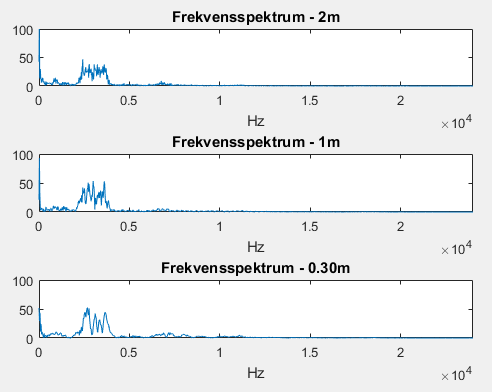
\includegraphics[width = 300pt]{Img/Frekvens.PNG}
\caption{Frekvensspektrum for de modtagne signaler}
\label{fig:Frekvensspektrum}
\end{figure}

Det kan ses at frekvensindholdet er klart størst i det forventede område (2000Hz-3500Hz). Der skal gøres opmærksom på at frekvensindholdet ikke er normaliseret, da det på denne måde var nemmere at se det relevante frekvensindhold. Udover det ønskede signal kan det ses at der ligger en del støj omkring de 7-8kHz. Dette er sandsynligvis lydforureningen, da vores signaler var optaget i et normalt klasseværelse med mange mennesker i.

Dernæst har vi krydskorreleret signalerne for at finde tidsforsinkelsen fra det originale signal til det reflekterede signal. Denne findes som afstanden imellem den største bølgetop i hhv. bølgen for det originale signal og bølgen for det reflekterede signal.

Krydskorrelationen er udregnet som:

\begin{figure}[H]
\centering
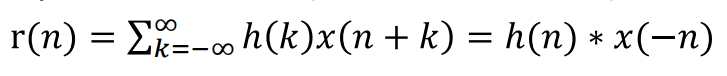
\includegraphics[width = 300pt]{Img/Krydskorrelation.PNG}
\caption{Formel for krydskorrelation}
\label{fig:Frekvensspektrum}
\end{figure}

Hvor r(n) er selve krydskorrelationen, h er det originale signal og x er det modtagne signal.

I MATLAB er det implementeret med følgende algoritme:

\begin{figure}[H]
\centering
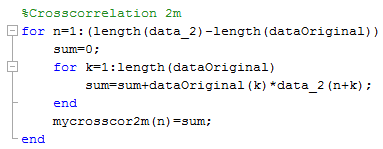
\includegraphics[width = 300pt]{Img/Matlab.PNG}
\caption{Krydskorrelation imlementeret i matlab}
\label{fig:Matlab}
\end{figure}

Nedenfor ses vores resultater.

\begin{figure}[H]
\centering
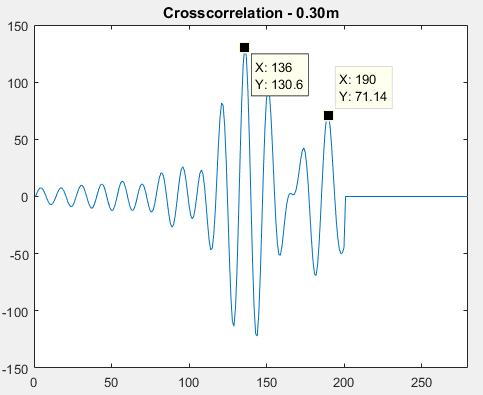
\includegraphics[width = 300pt]{Img/03m.PNG}
\caption{Krydskorrelation resultat for 0.3 meter}
\label{fig:03m}
\end{figure}

\begin{figure}[H]
\centering
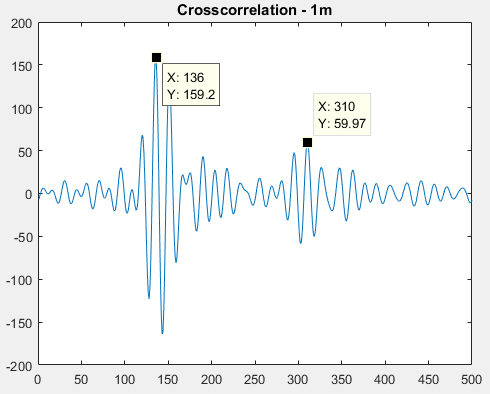
\includegraphics[width = 300pt]{Img/1m.PNG}
\caption{Krydskorrelation resultat for 1 meter}
\label{fig:1m}
\end{figure}

\begin{figure}[H]
\centering
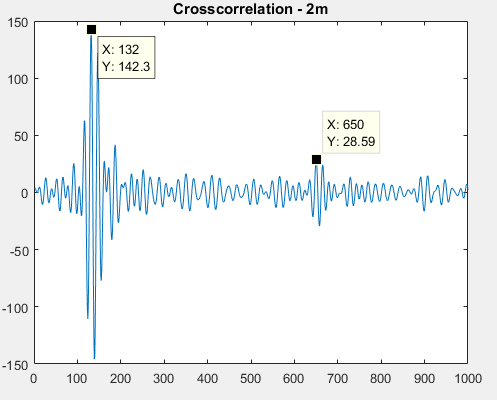
\includegraphics[width = 300pt]{Img/2m.PNG}
\caption{Krydskorrelation resultat for 2 meter}
\label{fig:2m}
\end{figure}

Afstanden til den første bølgetop repræsenterer afstanden imellem vores mikrofon og vores højtaler. Afstanden imellem den første bølgetop og den anden bølgetop repræsenterer den dobbelte afstand mellem mikrofon og væggen (da lyden skal frem OG tilbage). Ganger vi forsinkelsen i antal samples med vores udregnede meter pr. samples får vi følgende resultater:

\begin{figure}[H]
\centering
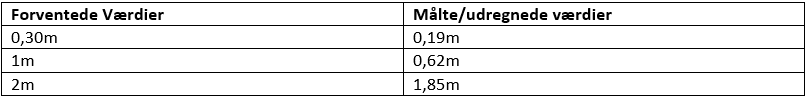
\includegraphics[width = 370pt]{Img/Resultater.PNG}
\caption{Udregnet afstand på baggrund af krydskorrelation}
\label{fig:Resultater}
\end{figure}


